\section{Tutorial}
\label{section:tutorial}
\setcounter{footnote}{0}

Here's a tutorial walk-through of some small projects with
Infernal. This should suffice to get you started on work of your own,
and you can (at least temporarily) skip the rest of the Guide,
such as all the nitty-gritty details of available command line
options.

\subsection {The programs in Infernal}


\begin{tabular}{ll}
\multicolumn{2}{c}{\textbf{Core programs}}\\
 & \\ 
\textbf{cmbuild}     & Build a covariance model from an input multiple alignment.\\
\textbf{cmcalibrate} & Calibrate E-value parameters for a covariance model.\\
\textbf{cmsearch}    & Search a covariance model against a sequence database.\\
\textbf{cmscan}      & Search a sequence against a covariance model database.\\
\textbf{cmalign}     & Make a multiple alignment of many sequences to a common covariance model.\\
 & \\ 
\multicolumn{2}{c}{\textbf{Other utilities}}\\ 
 & \\ 
\textbf{cmconvert} & Convert CM formats to/from Infernal v1.1 format.\\ 
\textbf{cmemit}    & Generate (sample) sequences from a covariance model.\\
\textbf{cmfetch}   & Get a covariance model by name or accession from a CM database.\\
\textbf{cmpress}   & Format a CM database into a binary format for \prog{cmscan}.\\
\textbf{cmstat}    & Show summary statistics for each model in a CM database.\\ 
\end{tabular} \\
\\

In this section, we'll show examples of running each of these
programs, using examples in the \ccode{tutorial/} subdirectory of the
distribution.

\subsection{Files used in the tutorial}

The subdirectory \prog{/tutorial} in the Infernal distribution contains the
files used in the tutorial, as well as a number of examples of various
file formats that Infernal reads. The important files for the tutorial
are:

\begin{sreitems}{\emprog{mrum-genome.fa}}
\item[\prog{tRNA5.sto}] A multiple alignment of five tRNA
  sequences. This file is a simple example of \emph{Stockholm
    format} that Infernal uses for structurally-annotated alignments.
%
\item[\prog{tRNA5.c.cm}] A calibrated version of a model built from
  \prog{tRNA5.sto}, included to save time. 
%
\item[\prog{mrum-genome.fa}]: the 3 Mb genome of the methanogenic archeaon 
  \emph{Methanobrevibacter ruminantium}, in
  FASTA format, downloaded from the NCBI Nucleotide database
  (accession: NC\_13790.1). 
%
\item[\prog{toalign.3.fa}] Three tRNA sequences
  in unaligned FASTA format.
%
\item[\prog{toalign.1trunc.fa}] A truncated tRNA sequence, actually
  the first sequence from \prog{toalign.3.fa} with some 5' and 3'
  residues removed to demonstrate alignment of truncated
  sequences.
%
\item[\prog{toalign.1.fa}] The first tRNA sequence from toalign.3.fa.
\end{sreitems}

\subsection{Searching a sequence database with a single covariance model}

\subsubsection{Step 1: build a covariance model with cmbuild}

Infernal starts with a multiple sequence alignment file that you
provide. It must be in Stockholm format and must include consensus
secondary structure annotation. The file \prog{tutorial/tRNA5.sto} is
an example of a simple Stockholm file. It is shown below, with a
secondary structure of the first sequence shown to the right for
reference (yeast Phe tRNA, labeled as ``tRNA1'' in the file):

\vspace{1em}
\begin{minipage}{4.7in}
\begin{sreoutput}[xleftmargin=0em]
# STOCKHOLM 1.0

tRNA1             GCGGAUUUAGCUCAGUUGGG.AGAGCGCCAGACUGAAGAUCUGGAGGUCC
tRNA2             UCCGAUAUAGUGUAAC.GGCUAUCACAUCACGCUUUCACCGUGGAGA.CC
tRNA3             UCCGUGAUAGUUUAAU.GGUCAGAAUGGGCGCUUGUCGCGUGCCAGA.UC
tRNA4             GCUCGUAUGGCGCAGU.GGU.AGCGCAGCAGAUUGCAAAUCUGUUGGUCC
tRNA5             GGGCACAUGGCGCAGUUGGU.AGCGCGCUUCCCUUGCAAGGAAGAGGUCA
#=GC SS_cons      <<<<<<<..<<<<.........>>>>.<<<<<.......>>>>>.....<

tRNA1             UGUGUUCGAUCCACAGAAUUCGCA
tRNA2             GGGGUUCGACUCCCCGUAUCGGAG
tRNA3             GGGGUUCAAUUCCCCGUCGCGGAG
tRNA4             UUAGUUCGAUCCUGAGUGCGAGCU
tRNA5             UCGGUUCGAUUCCGGUUGCGUCCA
#=GC SS_cons      <<<<.......>>>>>>>>>>>>.
//
\end{sreoutput}
\end{minipage}
\begin{minipage}{1.5in}
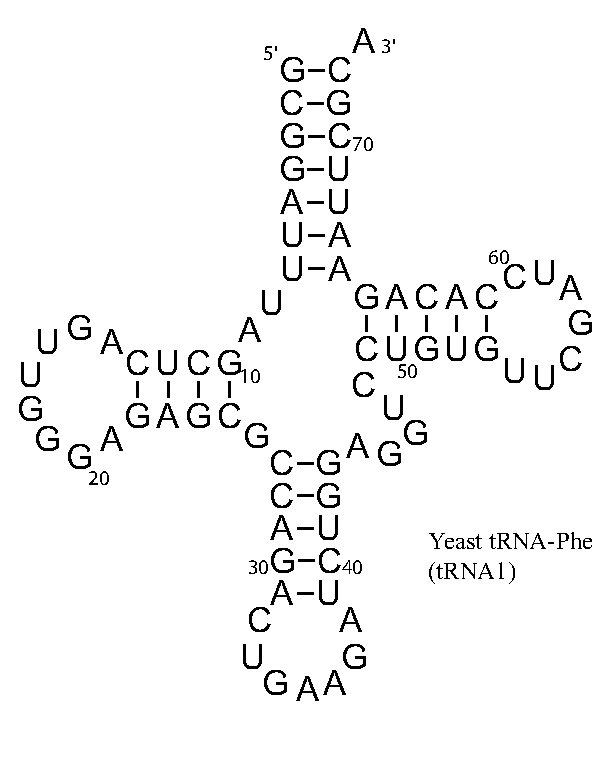
\includegraphics[scale=0.4]{Figures/trna1-DF6280}
\end{minipage}
\vspace{1em}

This is a simple example of a multiple RNA sequence alignment with
secondary structure annotation, in \emph{Stockholm format}. Stockholm
format, the native alignment format used by \software{hmmer} and
Infernal and the \database{Pfam} and \database{Rfam} databases, is
documented in detail later in the guide in
section~\ref{section:stockholm}.

For now, what you need to know about the key features of the input file is:
\begin{itemize}
\item The alignment is in an interleaved format.
Lines consist of a name, followed by an aligned sequence;
long alignments are split into blocks separated by blank lines.
\item Each sequence must have a unique name that has zero spaces in it. (This is important!)
\item For residues, any one-letter IUPAC nucleotide code is accepted,
      including ambiguous nucleotides. Case is ignored; residues
      may be either upper or lower case.
\item Gaps are indicated by the characters ., \_, -, or \verb+~+.
      (Blank space is not allowed.)
\item A special line starting with {\small\verb+#=GC SS_cons+} indicates
      the secondary structure consensus. Gap characters annotate
      unpaired (single-stranded) columns. Base pairs are indicated
      by any of the following pairs: \verb+<>+, \verb+()+, \verb+[]+,
      or \verb+[]+. No pseudoknots are allowed; the
      open/close-brackets notation is only unambiguous for strictly
      nested base-pairing interactions.
      For more on secondary structure annotation see
      section~\ref{section:wuss}.
\item The alignment begins with the special tag line
      {\small\verb+# STOCKHOLM 1.0+}, and ends with {\small\verb+//+}.
      Stockholm alignments
      can be concatenated to create an alignment database flatfile
      containing many alignments.
\end{itemize}

The \prog{cmbuild} command builds a covariance model from an alignment (or
CMs for each of many alignments in a Stockholm file), and saves the
CM(s) in a file. For example, type:

\user{cmbuild tRNA5.cm tutorial/tRNA5.sto}

and you'll see some output that looks like:

% tutorial regression: tRNA5-build.out
\begin{sreoutput}
# cmbuild :: covariance model construction from multiple sequence alignments
# INFERNAL 1.1 (May 2012)
# Copyright (C) 2012 Howard Hughes Medical Institute.
# Freely distributed under the GNU General Public License (GPLv3).
# - - - - - - - - - - - - - - - - - - - - - - - - - - - - - - - - - - - -
# CM file:                                            tRNA5.cm
# alignment file:                                     tRNA5.sto
# - - - - - - - - - - - - - - - - - - - - - - - - - - - - - - - - - - - -
#                                                                      rel entropy
#                                                                      -----------
# idx    name                     nseq eff_nseq   alen  clen  bps bifs    CM   HMM description
# ------ -------------------- -------- -------- ------ ----- ---- ---- ----- ----- -----------
       1 tRNA5                       5     3.73     74    72   21    2 0.783 0.489 
#
# CPU time: 0.37u 0.00s 00:00:00.37 Elapsed: 00:00:00.38
\end{sreoutput}

If your input file had contained more than one alignment, you'd get
one line of output for each model. The information on these lines is
almost self-explanatory. The \prog{tRNA5} alignment consisted of 5
sequences with 74 aligned columns. Infernal turned it into a model of
72 consensus positions, which means it defined 2 gap-containing
alignment columns to be insertions relative to consensus. The 5
sequences were only counted as an ``effective'' total sequence number
(\prog{eff\_nseq}) of 3.73. The model includes 21 basepairs and two
bifurcations. The model ended up with a relative entropy per position
(\prog{rel entropy, CM}; information content) of 0.783 bits. If the
secondary structure information of the model were ignored the relative
entropy per position (\prog{rel entropy, HMM}) would be 0.489 bits.

This output format is rudimentary. Infernal knows quite a bit more
information about what it's done to build this CM, but it's not
displaying it. You don't need to know more to be able to use the
model, so we can press on here. Model construction is described in
more detail in section~\ref{section:cmbuild}.

The new CM was saved to \prog{tRNA5.cm}. You can look at it
(e.g. \prog{> more tRNA5.cm}) if you like, but it isn't really designed
to be human-interpretable. You can treat \prog{.cm} files as compiled
models of your RNA alignment. The Infernal ASCII save file format is
defined in Section~\ref{section:formats}.

\begin{srefaq}{Can I build a model from a single sequence?}
Yes. But a structure for the sequence must still be supplied.
With single sequences, you can also build a \software{rsearch} \cite{KleinEddy03} CM 
using the \prog{--rsearch} option to \prog{cmbuild}. There's more on
this in a later section.
\end{srefaq}

\begin{srefaq}{Can I build a model from unaligned sequences?}
In principle, CMs can be trained from unaligned sequences;
however, this functionality is not yet implemented in Infernal.  I
recommend CLUSTALW as an excellent, freely available multiple sequence
alignment program. The original \prog{covet} CM training
program from COVE, the predecessor of Infernal is also
still available by
\url{ftp://selab.janelia.org/pub/software/cove/cove-2.4.4.tar.Z}.
\end{srefaq}

\subsubsection{Step 2: calibrate the model with cmcalibrate}

The model calibration step is required if you plan to use the model
for database searches with \prog{cmsearch} or \prog{cmscan}. In this
step, statistical parameters necessary for reporting E-values
(expectation values) are estimated and stored in the CM file.  When
\prog{cmsearch} or \prog{cmscan} is later used for a database search
and a hit with score $x$ is found, the E-value of that hit is the
number of hits expected to score $x$ or more just by chance in a
sequence database of this size. 

\emph{Importantly, if you're not going to use a model for database
search, there is no need to calibrate it.} For example, if you are
only going to build alignments with a model of a large family like
small subunit ribosomal RNA, don't waste time calibrating
it. \prog{cmsearch} and \prog{cmscan} are the only Infernal programs
that use E-values, so if you're not going to use them, don't
calibrate your model.

Unfortunately, CM calibration takes a long time because fairly long
random sequences must be searched to determine the expected
distribution of hit scores against nonhomologous sequences, and none
of the search acceleration heuristics described in
section~\ref{section:pipeline} can be used because they rely on
detecting primary sequence similarity which is absent in random
sequence. 

The amount of time required for calibration varies widely, but
depends mainly on the size of the RNA family being modeled.
%\prog{cmcalibrate} will predict it's own runtime (and finish
%without performing the calibration) if the \prog{--forecast} option is
%used. 
So you can know what kind of a wait you're in for, the
\prog{cmcalibrate} has a \prog{--forecast} option which reports an
estimate of the running time. To get an estimate for the tRNA model, do:

\user{cmcalibrate --forecast tRNA5.cm}\\

You should see something like this:

% tutorial regression: tRNA5-calibrate-fc.out
\begin{sreoutput}
# cmcalibrate :: fit exponential tails for CM E-values
# INFERNAL 1.1 (May 2012)
# Copyright (C) 2012 Howard Hughes Medical Institute.
# Freely distributed under the GNU General Public License (GPLv3).
# - - - - - - - - - - - - - - - - - - - - - - - - - - - - - - - - - - - -
# CM file:                                     tRNA5.cm
# forecast mode (no calibration):              on (8 CPUs)
# - - - - - - - - - - - - - - - - - - - - - - - - - - - - - - - - - - - -
#
# Forecasting running time for CM calibration(s) on 8 cpus:
#
#                          predicted
#                       running time
# model name            (hr:min:sec)
# --------------------  ------------
  tRNA5                     00:04:43
#
# CPU time: 0.20u 0.00s 00:00:00.20 Elapsed: 00:00:00.20
\end{sreoutput}

The header comes first, telling you what program you ran, on what file
and with what options. This calibration will use 8 CPUs, your output
may vary depending on how many cores you have available on the machine
you're using. (If you are planning to use MPI to parallelize the
calibration (see the Installation section), you can specify the number
of CPUs for the time estimate as \prog{<n>} with the \prog{--nforecast
<n>} option.) Using 8 CPUs, \prog{cmcalibrate} estimates the time
required for calibration on the machine I'm using at about five
minutes.

Feel free to perform the calibration yourself if you'd like (with the
command \prog{cmcalibrate tRNA5.cm}). However, we've included the file
\prog{tRNA5.c.cm}, an already calibrated version of \prog{tRNA5.cm},
for you to use if you don't want to wait. When we calibrated the
\prog{tRNA5.c.cm} file, the file was modified to include E-value
parameters. If you want to save time and skip the calibration, 
copy over the \prog{tRNA5.cm} file you just made with the calibrated
version:
 
\user{cp tRNA5.c.cm tRNA5.cm}\\
 
\subsubsection{Step 3: search a sequence database with cmsearch}

You can now use your tRNA model to search for tRNA homologs in a
database. The file \prog{mrum-genome.fa} is the genome sequence of the
archaeon \emph{Methanobrevibacter rumanitium}. We'll use this file as
our database. To perform the search:

\user{cmsearch tRNA5.cm mrum-genome.fa}\\

As before, the first section is the header, telling you what program
your ran, on what, and with what options, as well as the name and size
of :

% tutorial regression: tRNA5-search.out
\begin{sreoutput}
# cmsearch :: search CM(s) against a sequence database
# INFERNAL 1.1 (May 2012)
# Copyright (C) 2012 Howard Hughes Medical Institute.
# Freely distributed under the GNU General Public License (GPLv3).
# - - - - - - - - - - - - - - - - - - - - - - - - - - - - - - - - - - - -
# query CM file:                         tRNA5.cm
# target sequence database:              mrum-genome.fa
# - - - - - - - - - - - - - - - - - - - - - - - - - - - - - - - - - - - -
Query:       tRNA5  [CLEN=72]
\end{sreoutput}

The second section is a list of ranked top hits (sorted by E-value,
most significant hit first):

% tutorial regression: tRNA5-search.out
\begin{sreoutput}
 rank     E-value  score  bias  sequence                        start     end   mdl trunc   gc  description
 ----   --------- ------ -----  ----------------------------- ------- -------   --- ----- ----  -----------
  (1) !   1.3e-18   71.5   0.0  gi|288559258|ref|NC_013790.1|  362026  361955 -  cm    no 0.50  Methanobrevibacter ruminantium M1 chromosome, 
  (2) !   3.3e-18   70.2   0.0  gi|288559258|ref|NC_013790.1| 2585265 2585193 -  cm    no 0.60  Methanobrevibacter ruminantium M1 chromosome, 
  (3) !     9e-18   68.8   0.0  gi|288559258|ref|NC_013790.1|  762490  762562 +  cm    no 0.67  Methanobrevibacter ruminantium M1 chromosome, 
  (4) !     9e-18   68.8   0.0  gi|288559258|ref|NC_013790.1| 2041704 2041632 -  cm    no 0.67  Methanobrevibacter ruminantium M1 chromosome, 
  (5) !   2.5e-17   67.4   0.0  gi|288559258|ref|NC_013790.1| 2351254 2351181 -  cm    no 0.62  Methanobrevibacter ruminantium M1 chromosome, 
  (6) !     3e-17   67.2   0.0  gi|288559258|ref|NC_013790.1|  735136  735208 +  cm    no 0.59  Methanobrevibacter ruminantium M1 chromosome, 
  (7) !   5.2e-17   66.4   0.0  gi|288559258|ref|NC_013790.1| 2186013 2185941 -  cm    no 0.53  Methanobrevibacter ruminantium M1 chromosome, 
  (8) !   1.6e-16   64.8   0.0  gi|288559258|ref|NC_013790.1| 2350593 2350520 -  cm    no 0.66  Methanobrevibacter ruminantium M1 chromosome, 
  (9) !   2.8e-16   64.1   0.0  gi|288559258|ref|NC_013790.1| 2585187 2585114 -  cm    no 0.59  Methanobrevibacter ruminantium M1 chromosome, 
 (10) !   9.1e-16   62.5   0.0  gi|288559258|ref|NC_013790.1|  662185  662259 +  cm    no 0.61  Methanobrevibacter ruminantium M1 chromosome, 
 (11) !   1.2e-15   62.1   0.0  gi|288559258|ref|NC_013790.1|  360887  360815 -  cm    no 0.55  Methanobrevibacter ruminantium M1 chromosome, 
 (12) !   1.6e-15   61.7   0.0  gi|288559258|ref|NC_013790.1| 2350984 2350911 -  cm    no 0.53  Methanobrevibacter ruminantium M1 chromosome, 
 (13) !   3.3e-15   60.7   0.0  gi|288559258|ref|NC_013790.1| 2186090 2186019 -  cm    no 0.54  Methanobrevibacter ruminantium M1 chromosome, 
 (14) !   4.1e-15   60.4   0.0  gi|288559258|ref|NC_013790.1| 2680159 2680233 +  cm    no 0.67  Methanobrevibacter ruminantium M1 chromosome, 
 (15) !   7.9e-15   59.5   0.0  gi|288559258|ref|NC_013790.1| 2749839 2749768 -  cm    no 0.53  Methanobrevibacter ruminantium M1 chromosome, 
 (16) !   7.9e-15   59.5   0.0  gi|288559258|ref|NC_013790.1| 2749945 2749874 -  cm    no 0.53  Methanobrevibacter ruminantium M1 chromosome, 
 (17) !   9.8e-15   59.2   0.0  gi|288559258|ref|NC_013790.1|  361676  361604 -  cm    no 0.51  Methanobrevibacter ruminantium M1 chromosome, 
 (18) !     1e-14   59.2   0.0  gi|288559258|ref|NC_013790.1| 2585073 2584999 -  cm    no 0.60  Methanobrevibacter ruminantium M1 chromosome, 
 (19) !   1.1e-14   59.1   0.0  gi|288559258|ref|NC_013790.1| 2130422 2130349 -  cm    no 0.59  Methanobrevibacter ruminantium M1 chromosome, 
 (20) !   1.2e-14   58.9   0.0  gi|288559258|ref|NC_013790.1|  546056  545947 -  cm    no 0.61  Methanobrevibacter ruminantium M1 chromosome, 
 (21) !   3.9e-14   57.3   0.0  gi|288559258|ref|NC_013790.1|  361915  361844 -  cm    no 0.42  Methanobrevibacter ruminantium M1 chromosome, 
 (22) !   5.1e-14   57.0   0.0  gi|288559258|ref|NC_013790.1|   97724   97795 +  cm    no 0.49  Methanobrevibacter ruminantium M1 chromosome, 
 (23) !   6.1e-14   56.7   0.0  gi|288559258|ref|NC_013790.1| 2350717 2350646 -  cm    no 0.68  Methanobrevibacter ruminantium M1 chromosome, 
 (24) !     8e-14   56.3   0.0  gi|288559258|ref|NC_013790.1| 1873887 1873815 -  cm    no 0.64  Methanobrevibacter ruminantium M1 chromosome, 
 (25) !   1.4e-13   55.6   0.0  gi|288559258|ref|NC_013790.1|  360730  360659 -  cm    no 0.40  Methanobrevibacter ruminantium M1 chromosome, 
 (26) !   3.5e-13   54.3   0.0  gi|288559258|ref|NC_013790.1| 2680310 2680384 +  cm    no 0.52  Methanobrevibacter ruminantium M1 chromosome, 
 (27) !   3.6e-13   54.3   0.0  gi|288559258|ref|NC_013790.1| 2664806 2664732 -  cm    no 0.60  Methanobrevibacter ruminantium M1 chromosome, 
 (28) !   3.6e-13   54.3   0.0  gi|288559258|ref|NC_013790.1|  361061  360989 -  cm    no 0.41  Methanobrevibacter ruminantium M1 chromosome, 
 (29) !   7.5e-13   53.3   0.0  gi|288559258|ref|NC_013790.1| 2130335 2130262 -  cm    no 0.55  Methanobrevibacter ruminantium M1 chromosome, 
 (30) !   7.6e-13   53.3   0.0  gi|288559258|ref|NC_013790.1| 2151672 2151745 +  cm    no 0.65  Methanobrevibacter ruminantium M1 chromosome, 
 (31) !   2.9e-12   51.4   0.0  gi|288559258|ref|NC_013790.1|  319297  319370 +  cm    no 0.62  Methanobrevibacter ruminantium M1 chromosome, 
 (32) !   3.7e-12   51.1   0.0  gi|288559258|ref|NC_013790.1|  361753  361679 -  cm    no 0.55  Methanobrevibacter ruminantium M1 chromosome, 
 (33) !   3.8e-12   51.1   0.0  gi|288559258|ref|NC_013790.1|  360983  360912 -  cm    no 0.50  Methanobrevibacter ruminantium M1 chromosome, 
 (34) !   5.9e-12   50.5   0.0  gi|288559258|ref|NC_013790.1|  361456  361383 -  cm    no 0.50  Methanobrevibacter ruminantium M1 chromosome, 
 (35) !   7.4e-12   50.1   0.0  gi|288559258|ref|NC_013790.1|  362798  362727 -  cm    no 0.51  Methanobrevibacter ruminantium M1 chromosome, 
 (36) !   8.7e-12   49.9   0.0  gi|288559258|ref|NC_013790.1|  917722  917793 +  cm    no 0.61  Methanobrevibacter ruminantium M1 chromosome, 
 (37) !   1.1e-11   49.7   0.0  gi|288559258|ref|NC_013790.1| 2583869 2583798 -  cm    no 0.51  Methanobrevibacter ruminantium M1 chromosome, 
 (38) !   1.3e-11   49.4   0.0  gi|288559258|ref|NC_013790.1|  362324  362252 -  cm    no 0.51  Methanobrevibacter ruminantium M1 chromosome, 
 (39) !   1.3e-11   49.3   0.0  gi|288559258|ref|NC_013790.1|  360811  360740 -  cm    no 0.42  Methanobrevibacter ruminantium M1 chromosome, 
 (40) !   4.3e-11   47.7   0.0  gi|288559258|ref|NC_013790.1| 1160526 1160609 +  cm    no 0.60  Methanobrevibacter ruminantium M1 chromosome, 
 (41) !   9.8e-11   46.6   0.0  gi|288559258|ref|NC_013790.1|  362403  362331 -  cm    no 0.49  Methanobrevibacter ruminantium M1 chromosome, 
 (42) !   1.1e-10   46.5   0.0  gi|288559258|ref|NC_013790.1| 2327124 2327042 -  cm    no 0.63  Methanobrevibacter ruminantium M1 chromosome, 
 (43) !   1.2e-10   46.4   0.0  gi|288559258|ref|NC_013790.1|  995344  995263 -  cm    no 0.49  Methanobrevibacter ruminantium M1 chromosome, 
 (44) !   2.3e-10   45.5   0.0  gi|288559258|ref|NC_013790.1|  256772  256696 -  cm    no 0.57  Methanobrevibacter ruminantium M1 chromosome, 
 (45) !   2.5e-10   45.3   0.0  gi|288559258|ref|NC_013790.1| 2584830 2584758 -  cm    no 0.64  Methanobrevibacter ruminantium M1 chromosome, 
 (46) !   6.1e-10   44.1   0.0  gi|288559258|ref|NC_013790.1| 2351071 2350997 -  cm    no 0.59  Methanobrevibacter ruminantium M1 chromosome, 
 (47) !   6.5e-10   44.0   0.0  gi|288559258|ref|NC_013790.1|  362552  362482 -  cm    no 0.55  Methanobrevibacter ruminantium M1 chromosome, 
 (48) !   5.2e-09   41.2   0.0  gi|288559258|ref|NC_013790.1| 1064775 1064858 +  cm    no 0.63  Methanobrevibacter ruminantium M1 chromosome, 
 (49) !   1.2e-08   40.0   0.0  gi|288559258|ref|NC_013790.1|  361222  361150 -  cm    no 0.45  Methanobrevibacter ruminantium M1 chromosome, 
 (50) !   1.2e-08   40.0   0.0  gi|288559258|ref|NC_013790.1|  361369  361297 -  cm    no 0.60  Methanobrevibacter ruminantium M1 chromosome, 
 (51) !   4.8e-08   38.1   0.0  gi|288559258|ref|NC_013790.1|  361596  361513 -  cm    no 0.61  Methanobrevibacter ruminantium M1 chromosome, 
 (52) !   3.2e-07   35.5   0.0  gi|288559258|ref|NC_013790.1| 1913310 1913227 -  cm    no 0.64  Methanobrevibacter ruminantium M1 chromosome, 
 (53) !   2.6e-06   32.7   0.0  gi|288559258|ref|NC_013790.1|  363464  363381 -  cm    no 0.51  Methanobrevibacter ruminantium M1 chromosome, 
 (54) !     3e-06   32.5   0.0  gi|288559258|ref|NC_013790.1| 2584954 2584872 -  cm    no 0.58  Methanobrevibacter ruminantium M1 chromosome, 
 ------ inclusion threshold ------
 (55) ?     0.027   20.0   0.0  gi|288559258|ref|NC_013790.1|  363803  363716 -  cm    no 0.50  Methanobrevibacter ruminantium M1 chromosome, 
 (56) ?       3.4   13.4   0.0  gi|288559258|ref|NC_013790.1|  984373  984304 -  cm    no 0.53  Methanobrevibacter ruminantium M1 chromosome, 
\end{sreoutput}

The first number is the rank of each hit (it appears in parantheses to
make it easy to jump to/from an entry in the hit list and the hit
alignment section, described later). Next comes either a \ccode{!} or
\ccode{?} symbol and then the \emph{E-value} of the hit.  The E-value
is the statistical significance of the hit: the number of hits we'd
expect to score this highly in a database of this size (total number
of nucleotides) if the database contained only nonhomologous random
sequences. The lower the E-value, the more significant the hit.  The
\ccode{!} or \ccode{?} that precedes the E-value indicates whether the
hit does (\ccode{!}) or does not (\ccode{?}) satisfy the inclusion
threshold for the search.  Inclusion thresholds are used to determine
what matches should be considered to be ``true'', as opposed to
reporting thresholds that determine what matches will be reported
(often including the top of the noise, so you can see what interesting
sequences might be getting tickled by your search). By default,
inclusion thresholds usually require an E-value of 0.01 or less, and
reporting E-value thresholds are set to 10.0, but these can be changed
(see the manual page for \prog{cmsearch} in
section\ref{section:manpages}).

The E-value is based on the \emph{bit score}, which is in the next
column. This is the log-odds score for the hit. Some people like to
see a bit score instead of an E-value, because the bit score doesn't
depend on the size of the sequence database, only on the covariance
model and the target sequence.

The next number, the \emph{bias}, is a correction term for biased
sequence composition that has been applied to the sequence bit
score. Infernal uses an alternative null model we call \emph{null3},
described more in section\label{section:null3}, to determine the bias
bit score correction. The bias correction is often very small and is
only reported to one decimal place, after rounding. For all hits in
this example search the bias column reads 0.0 bits, indicating that
the correction is less than 0.05 bits. On very biased sequences this
correction can become significant and is helpful for lowering the
score of high-scoring false positives that achieve high scores solely
due to their biased composition. 

Next comes the target sequence name the hit is in, and the start and
end positions of the hit within the sequence. Hits can occur on either
the top (Watson) or bottom (Crick) strand of the target
sequence\footnote{You can search either only the top strand with the
\prog{--toponly} or bottom strand with the \prog{--bottomonly} options
to \prog{cmsearch} and \prog{cmscan}.}, so the start position may be
less than (if hit is on the top strand) or greater than (if hit is on
the reverse strand) the end position. After the end position, comes a single
\ccode{+} or \ccode{-} symbol, indicating whether the hit is on the
top (\ccode{+}) or bottom (\ccode{-}) strand.

After the strand symbol comes the model field, which indicates whether
the hit was found using either the CM (\prog{cm}) or a profile HMM
built from the CM (\prog{hmm}). This field is necessary because for
models with zero basepairs, \prog{cmsearch} (and \prog{cmscan}) use a
profile HMM instead of a CM for final hit scoring. This is done for
reasons of speed and efficiency, because profile HMM algorithms are
more efficient than CM ones and a CM with zero basepairs is
essentially equivalent to a profile HMM. In this example, since our
tRNA model does include basepairs, \prog{cmsearch} used a CM to score
all hits and so all hits have \prog{cm} for this column. There's an
example later in the tutorial of hits found with a profile HMM.

The next column indicates whether the hit is \emph{truncated} or
not. Infernal uses special versions of its CM dynamic programming
algorithms to allow detection of structural RNAs that have been
truncated due to missing data at the beginning and/or end of a target
sequence. Truncated hits are most common in databases that include
single reads from shotgun sequencing projects. Since our database is a
complete genome, we don't expect any hits to be truncated due to
missing data. For all hits the``trunc'' column reads
``no'' indicating that, as expected, none of the hits are
truncated. There are examples of truncated hits in the next exercise
which uses \prog{cmscan}. Section\prog{section:trunc} describes how
Infernal detects and aligns truncated hits in more detail.

The next column reports the GC fraction of the hit. This is the
fraction of residues in the target sequence hit that are either
\prog{G} or \prog{C} residues. The GC fraction is included as an
additional indication of the level of sequence bias of the hit. Some
expert users may be aided by this number when determining if they
believe a hit is a real homolog or a false positive.

Finally comes the description of the sequence, if any. This
description is propogated from the input target sequence file.

After the hit list comes the hit alignments section. Each hit in 
the hit list will have a corresponding entry in this section, in the
same order. As an illustrative example, let's take a look at
hit number 43. First, take a look at the first four lines for this
hit: 

% tutorial regression: tRNA5-search.out
\begin{sreoutput}
>> gi|288559258|ref|NC_013790.1|  Methanobrevibacter ruminantium M1 chromosome, complete genome
 rank     E-value  score  bias mdl mdl from   mdl to       seq from      seq to       acc trunc   gc
 ----   --------- ------ ----- --- -------- --------    ----------- -----------      ---- ----- ----
 (43) !   1.2e-10   46.4   0.0  cm        1       72 []      995344      995263 - .. 0.93    no 0.49
\end{sreoutput}

The first line of each hit alignment begins with \ccode{>>} followed
by a single space, the name of the target sequence, then two spaces
and the description of the sequence, if any. Next comes a set of
tabular fields that is partially redundant with the information in the
hit list. The first five columns are the same as in the hit list. The
next column reports the type of model used for the alignment, as
described above for the hit list. The next four columns report the
boundaries of the alignment with respect to the query model (``mdl
from'' and ``mdl to'') and the target sequence (``seq from'' and ``seq
to''). Following the ``seq to'' column is a \ccode{+} or \ccode{-}
symbol indicating whether the hit is on the top (\ccode{+}) or bottom
(\ccode{-}) strand.

It's not immediately easy to tell from the ``to'' coordinate whether
the alignment ended internally in the query model or target sequence,
versus ran all the way (as in a full-length global alignment) to the
end(s). To make this more readily apparent, with each pair of query
and target endpoint coordinates, there's also a little symbology. For
the normal case of a non-truncated hit: \prog{..} means both ends of
the alignment ended internally, and \prog{[]} means both ends of the
alignment were full-length flush to the ends of the query or target,
and \prog{[.}  and \prog{.]} mean only the left (5') or right (3') end
was flush/full length.  For truncated hits, the symbols are the same
except that either the first and/or the second symbol will be a
\prog{~} for the query and target. If the first symbol is \prog{~}
then the left end of the alignment is truncated because the 5' end of
the hit is predicted to be missing (extend beyond the beginning of the
target sequence). Similarly, if the second symbol is \prog{~} then the
right end of the alignment is truncated because the 3' end of the hit
is predicted to be missing (extend beyond the end of the target
sequence). These two symbols occur just after the ``md to'' column for
the query, and after the strand \ccode{+} or \ccode{-} symbol for the
target sequence.

The next column is labeled ``acc'' and is the average posterior
probability of the aligned target sequence residues; effectively, the
expected accuracy per residue of the alignment.

The final two columns indicate whether the hit is truncated or not and
the GC fraction of the hit. These are redundant with the columns of
the same name in the hit list, described above.

Next comes the alignment display. This is an ``optimal
posterior accuracy'' alignment \cite{Holmes98}, which means it is the
alignment with the maximal summed posterior probability of all
aligned residues. Take a look at the alignment for hit number 43:

% tutorial regression: tRNA5-search.out
\begin{sreoutput}
                                                   v         v                                                    NC
                                       (((((((,,<<<<______.._>>>>,<<<<<_______>>>>>,,,........,,<<<<<_______>>>>> CS
                          tRNA5      1 gCcggcAUAGcgcAgUGGu..AgcgCgccagccUgucAagcuggAGg........UCCgggGUUCGAUUCcccG 64    
                                       :::G:CAUAGCG AG GGU  A CGCG:CAG:CU +++A:CUG: G+        UC:GGGGUUCGA UCCCC:
  gi|288559258|ref|NC_013790.1| 995344 AGAGACAUAGCGAAGCGGUcaAACGCGGCAGACUCAAGAUCUGUUGAuuaguucuUCAGGGGUUCGAAUCCCCU 995271
                                       **********************************************9444444445****************** PP

                                                NC
                                       ))))))): CS
                          tRNA5     65 UgccgGca 72    
                                       UG:C:::A
  gi|288559258|ref|NC_013790.1| 995270 UGUCUCUA 995263
                                       ******** PP
\end{sreoutput}

The alignment is broken up into blocks, in this case two.
Each block consists of six lines. If your model was built with the
\ccode{--hand} option in \prog{cmbuild}, then a seventh line will be
displayed with RF annotation, as shown in an example later in the
tutorial. If the model used for the alignment was an HMM (the ``mdl''
column reads ``hmm''), as shown in an example later in the tutorial,
then only five columns will be displayed (the \ccode{NC} line will be
absent). 

Start by looking at the second line which ends with \ccode{CS}.  The
line shows the predicted secondary structure of the target
sequence. The format is a little fancier and more informative than the
simple least-common-denominator format we used in the input alignment
file. It's designed to make it easier to see the secondary structure
by eye. The format is described in detail later
(section~\ref{section:wuss}; for now, here's all you need to
know. Basepairs in simple stem loops are annotated with \verb+<>+
characters. Basepairs enclosing multifurcations (multiple stem loops)
are annotated with \verb+()+, such as the tRNA acceptor stem in this
example. In more complicated structures, \verb+[]+ and \verb+{}+
annotations also show up, to reflect deeper nestings of
multifurcations. For single stranded residues, \verb+_+ characters
mark hairpin loops; \verb+-+ characters mark interior loops and
bulges; \verb+,+ characters mark single-stranded residues in
multifurcation loops; and \verb+:+ characters mark single stranded
residues external to any secondary structure. Insertions relative to
this consensus are annotated by a \verb+.+ character.

The line above the \ccode{CS} line ends with \ccode{NC} and marks
negative scoring non-canonical basepairs in the alignment with a
\ccode{v} character. All other positions of the alignment will be
blank\footnote{For anyone trying to parse this output, this means it
is possible for this line to be completely blank except for the
\ccode{NC} trailer.} More specifically, the following ten types of
basepairs which are assigned a negative score by the model at their
alignment positions will be marked with a \ccode{v}: \ccode{A:A},
\ccode{A:C}, \ccode{A:G}, \ccode{C:A}, \ccode{C:C}, \ccode{C:U},
\ccode{G:A}, \ccode{G:G}, \ccode{U:U}, and \ccode{U:C}. The \ccode{NC}
annotation makes it easy to quickly identify suspicious basepairs in
a hit. Importantly, the \ccode{NC} annotation will only be present in
CM hit alignments (``mdl'' column reads ``cm'') and will be absent in
HMM hit alignments (``mdl'' column reads ``hmm'') because basepairs
are not scored by an HMM.

The third line shows that consensus of the query model. The highest
scoring residue sequence is shown. Upper case residues are highly
conserved. Lower case residues are weakly conserved or unconserved.
Dots (\prog{.}) in this line indicate insertions in the target
sequence with respect to the model.

The fourth line shows where the alignment score is coming from. For a
consensus basepair, if the observed pair is the highest-scoring
possible pair according to the consensus, both residues are shown in
upper case; if a pair has a score of $\geq 0$, both residues are
annotated by : characters (indicating an acceptable compensatory
basepair); else, there is a space, indicating that a negative
contribution of this pair to the alignment score. Note that the 
\ccode{NC} line will only mark a subset of these negative scoring
pairs with a \ccode{v}, as discussed above.
For a single-stranded consensus residue, if the observed residue is
the highest scoring possibility, the residue is shown in upper case;
if the observed residue has a score of $\geq 0$, a \verb+++ character
is shown; else there is a space, indicating a negative contribution to
the alignment score. Importantly for HMM hits (``mdl'' column reads
``hmm''), \emph{all} positions are considered single stranded, since
an HMM does scores each half of a basepair independently.

The fifth line, beginning with \prog{gi|288559258|ref|NC\_013790.1} is
the target sequence. Dashes (\prog{-}) in this line indicate deletions
in the target sequence with respect to the model.

The bottom line is new to version 1.1 of Infernal. This represents the
posterior probability (essentially the expected accuracy) of each
aligned residue. A 0 means 0-5\%, 1 means 5-15\%, and so on; 9 means
85-95\%, and a \prog{*} means 95-100\% posterior probability. You can
use these posterior probabilities to decide which parts of the
alignment are well-determined or not. You'll often observe, for
example, that expected alignment accuracy degrades around locations of
insertion and deletion, which you'd intuitively expect.

After hit number 43, there's 13 more hit alignments for hits number 44
through 56. 

Finally, at the bottom of the file, you'll see some summary
statistics. For example, at the bottom of the tRNA search output,
you'll find something like:

\begin{sreoutput}
Internal CM pipeline statistics summary:
----------------------------------------
Query model(s):                                                  1  (72 consensus positions)
Target sequences:                                                1  (5874406 residues searched)
Target sequences re-searched for truncated hits:                 1  (360 residues re-searched)
Windows   passing  local HMM SSV           filter:           11197  (0.2108); expected (0.35)
Windows   passing  local HMM Viterbi       filter:                  (off)
Windows   passing  local HMM Viterbi  bias filter:                  (off)
Windows   passing  local HMM Forward       filter:             140  (0.002747); expected (0.005)
Windows   passing  local HMM Forward  bias filter:             139  (0.002728); expected (0.005)
Windows   passing glocal HMM Forward       filter:              88  (0.001973); expected (0.005)
Windows   passing glocal HMM Forward  bias filter:              88  (0.001973); expected (0.005)
Envelopes passing glocal HMM envelope defn filter:             101  (0.001358); expected (0.005)
Envelopes passing  local CM  CYK           filter:              60  (0.0007629); expected (0.0001)
Total CM hits reported:                                         56  (0.0007205); includes 0 truncated hit(s)

# CPU time: 1.86u 0.02s 00:00:01.88 Elapsed: 00:00:00.55
//
\end{sreoutput}

This gives you some idea of what's going on in Infernal's acceleration
pipeline. You've got one query CM, and the database has one target
%                                                       ^
sequence. The search examined 5,874,406 residues, even though the
actual target sequence length is only half that, because both the top
and bottom strand of each target is searched. 360 of those residues
were searched more than once in an effort to find truncated
hits. Ignore this for the moment, we'll revisit this later after
discussing the filter pipeline. 

\begin{comment}
In this case, these were the first and final 90 residues of each the
top and bottom strand. Infernal only re-searches sequence terminii
because it only expects truncated hits to occur at the ends of a
sequence, and based on the input alignment \prog{tRNA5.sto} used to
build a model, Infernal expects a hit to be at most 90 residues
long. Infernal's truncated hit detection strategy is discussed further
in the next tutorial section.
\end{comment}

Each sequence goes through a multi-stage filter pipeline of four
scoring algorithms called SSV, Viterbi, Forward, and CYK in order of
increasing sensitivity and increasing computational requirement.  The
filter pipeline is the topic of section~\ref{section:pipeline} of this
guide but briefly, SSV, Viterbi and Forward are profile
HMM algorithms which are more efficient than CM algorithms. These
three algorithms are the same ones used by HMMER3 and are the main
reason that version 1.1 of Infernal is so much faster than previous
versions. For these HMM stages, Infernal uses a filter profile HMM
that was constructed simultaneously with the CM, from the same
training alignment in \prog{cmbuild}, and stored in the CM file. CYK
is a CM scoring algorithm, so it's slow, but it is accelerated using
banded dynamic programming with bands derived from an HMM
alignment. Subsequences that survive all filters are finally scored
with the CM Inside algorithm, agains using HMM bands. Subsequences
that score sufficiently high with Inside are then aligned using the
optimal posterior accuracy algorithm and displayed.

The score thresholds for a subsequence surviving each HMM filter stage
are dependent on the size of the database, unlike in HMMER3. In
general, the larger the database the more strict the thresholds
are, because a hit must have a higher bit score to have a
significant E-value. 
\begin{comment}
The rationale for this is as follows: for a hit of a given bit
score the E-value increases with the database size making it harder to
distinguish from noise, so filters can be more strict for larger
databases because they can safely filter out higher scoring hits.
\end{comment}
In this case, the database is relatively small so the filter
thresholds have been set relatively loosely. The SSV filter has been
configured to allow subsequences with a P-value of $\leq 0.35$ through
%                                                        ^^^^
the SSV score filter (thus, if the database contained no homologs and
P-values were accurately calculated, the highest scoring 35\% of the
%                                           ^^^^
residues will pass the filter). Here, about 21\% of the database in
%                                           ^^^^
11,197 separate windows got through the SSV filter. For a database of
%^^^^^
this size, the local Viterbi filter is turned off.  The local Forward filter
is set to allow an expected 0.5\% of the database survive. Here about
%                           ^^^^
0.03\% survives in 140 windows. Next, each surviving window is checked
%^^^
to see if the target sequence is ``obviously'' so biased in its
composition that it's unlikely to be a true homolog. This is called
the ``bias filter'' and applying a bit score correction to previous
filter's score for each window and recomputing the P-value.
Exactly 1 of the 140 windows fails to pass the local Forward bias filter stage
%^^^^^^^^        ^^^
Next, the Forward algorithm is used to score each window again, but
this time with the HMM configured in glocal mode requiring a full
length alignment to the model\footnote{The use of glocal Forward is
another important difference between Infernal and HMMER3's (v3.0)
pipeline. HMMER v3.0 only uses local HMM algorithms.}  As with the
local stage, an expected 0.5\% of the database is expected to
survive. In this case, 88 of the 139 windows, comprising about 0.2\%
of the database, survive. The bias filter is run again, this time
applying a correction to the glocal Forward scores. For this search 0
windows are removed at this stage. The envelope definition stage is
next. This stage is very similar to the HMMER3 domain definition
stage, with the difference that the HMM is configured in glocal rather
than local mode. In this stage, the Forward and Backward algorithms
are used to identify zero or more hit envelopes in each window, where
each envelope contains one putative hit.  Often residues at the
beginning and ends of windows are determined to be nonhomologous and
are not included in the envelope. In this search, 101 envelopes are
defined within the 81 windows. Note that the envelopes comprise only
about 70\% of the residues from the 81 windows, indicated by the drop
of 0.1973\% to 0.1358\%. 

After hit envelopes have been defined with the filter HMM, the
remaining stages of the pipeline use the CM to score both the
conserved sequence and structure of each possible hit. First, the CYK
algorithm (which is the SCFG analog of the Viterbi HMM algorithm) is
used to determine the best scoring maximum likelihood alignment of any
subsequence in each envelope to the CM. If this alignment has a
P-value of less than $1e-4$ then the envelope survives to the final
round. The envelopes passed to the final stage may be shorter than
those examined during the CYK stage. Specifically, envelopes are
redefined as starting and ending at the first and final residues for
which at least one alignment exists with a P-value less than $1e-3$.

In the final round, the Inside algorithm (the SCFG analog of
the HMM Forward algorithm) is used to define
final hit boundaries and scores. Hits with scores above the reporting
threshold were output, as described above. In this search there were
56 such hits. 

Finally, the running time of the search is reported, in CPU time and
elapsed time. This search took about 1.86 seconds of elapsed (wall
%                                    ^^^^
clock time) (running with \ccode{--cpu 2} on two cores). 

\subsubsection{Truncated RNA detection}

Now, we come back to the topic of truncated hit detection.  As briefly
mentioned above, the pipeline statistics summary from our search above
reported that 360 residues were re-searched for truncated
hits. Infernal explicitly looks at the 5' and 3' ends of target
sequences using specialized algorithms for detection of truncated
hits, in which part of the 5' and/or 3' end of the actual full length
homologous sequence from the source organism's full genomic context is
missing in the input target sequence. Truncated hits will be most
common in sequence files consisting of unassembled sequencing
reads. In our search of the full archaeal genome above, no truncated
hits were found. However, there is an example of a truncated hit in
the \prog{cmscan} tutorial section below in a sequence from a
metagenomics sequencing survey.

Special dynamic programming algorithms are required for truncated hit
detection \cite{KolbeEddy09}, so sequences must be re-searched for
truncated hits after they are initially searched for standard
(non-truncated) hits. However, only the sequence ends must be
re-searched because Infernal assumes that only hits at sequence
terminus might be truncated. This is why our search above reported
that only 360 residues were re-searched for truncated hits. For each
model, an expected maximum length of a hit\footnote{The expected
maximum hit length is computed with the QDB algorithm
\cite{NawrockiEddy07} based on the transition probabilities of the
model by \prog{cmbuild} and is stored as the \ccode{W} parameter in
the CM file.}  is used to define the window length at the beginning
and end of each sequence which must be re-searched for truncated
hits. For our tRNA model the maximum expected length is 90, so
exactly 360 residues were re-searched: the first and final 90 residues
on the top strand, and the first and final 90 residues on the bottom
strand. 

There is one more aspect of truncated hit detection that is important
to point out. Because Infernal expects that hit truncation only occurs
at the ends of target sequences, 5' truncated hits are forced to
include the first residue of a target sequence, 3' truncated hits are
forced to include the final residue of a target sequence and 5' and 3'
truncated hits are forced to include the first and final residue of a
target sequence. 

The annotation of truncated hits in \prog{cmsearch} output is slightly
different than for standard hits. An example is shown and explained
in the next section below. 

\subsection{Searching a CM database with a query sequence}

The \prog{cmscan} program is for annotating all the different
known/detectable RNAs in a given sequence. It takes a single query
sequence and a CM database as input. The CM database might be Rfam,
for example, or another collection of your choice. \prog{cmscan} is
new to version 1.1 of Infernal. It is designed to be useful for
the analysis metagenomic datasets, in which one wants to know what
families of RNAs are represented in the sequence dataset.

\subsubsection{Step 1: create an CM database flatfile}

A CM ``database'' flatfile is simply a concatenation of individual CM
files. To create a database flatfile, you can either build and
calibrate individual CM files and concatenate them, or you can
concatenate Stockholm alignments and use \prog{cmbuild} to build an CM
database of all of them in one command, and then calibrate that
database with \prog{cmcalibrate}. Importantly, \prog{cmscan} can only
be used with calibrated CMs.

Let's create a tiny database called \prog{minifam.cm} containing the
tRNA model we've been working with, a 5S ribosomal RNA model, and a
Cobalamin riboswitch model. To save you time, calibrated versions of
the 5S and Cobalamin models are included in the \prog{tutorial/}
directory in the files \prog{5S\_rRNA.c.cm}, and
\prog{Cobalamin.c.cm}. These files were created using \prog{cmbuild}
and \prog{cmcalibrate} from the Rfam 10.1 seed alignments for 5S\_rRNA
(RF00001) and Cobalamin (RF00174). The third model is the tRNA model
from earlier in the tutorial (\prog{tutorial/tRNA5.c.cm}). In the
interest of time, we'll just concatenate the three provided files to
make the database:

\prog{cat tutorial/tRNA5.c.cm tutorial/5S\_rRNA.c.cm tutorial/Cobalamin.c.cm > minifam.cm}

\subsubsection{Step 2: compress and index the flatfile with cmpress}

The \prog{cmscan} program has to read a lot of CMs and their filter
HMMs in a hurry, and Infernal's ASCII flatfiles are bulky. To
accelerate this, \prog{cmscan} uses binary compression and indexing of
the flatfiles.  To use \prog{cmscan}, you must first compress and
index your CM database with the \prog{cmpress} program:

\user{cmpress minifam.cm}

This will quickly produce:

\begin{sreoutput}
Working...    done.
Pressed and indexed 3 CMs and p7 HMM filters (3 names and 2 accessions).
Covariance models and p7 filters pressed into binary file:  minifam.cm.i1m
SSI index for binary covariance model file:                 minifam.cm.i1i
Optimized p7 filter profiles (MSV part)  pressed into:      minifam.cm.i1f
Optimized p7 filter profiles (remainder) pressed into:      minifam.cm.i1p
\end{sreoutput}

and you'll see these four new binary files in the directory. 

The \prog{tutorial} directory includes a copy of the
\prog{minifam.cm} file, which has already been pressed, so there
are example binary files\\
\prog{tutorial/minifam.cm.i1\{m,i,f,p\}}
included in the tutorial.

Their format is ``proprietary'', which is an open source term of art
that means both ``We haven't found time to document them yet'' and ``We
still might decide to change them arbitrarily without telling you''.

\subsubsection{Step 3: search the CM database with cmscan}

Now we can analyze sequences using our CM database and
\prog{cmscan}. 

For example, the tutorial file \prog{tutorial/contrived.fa} includes X
sequences from a metagenomics dataset that includes soil samples and three
``whale fall'' carcasses \cite{Tringe05}. These sequences were
chosen because they include promising hits to the three models in
our toy CM database.

To scan the sequences with our database: 

\user{cmscan minifam.cm tutorial/contrived.fa}

The header and the first section of the output will look like:

% tutorial regression: contrived.cmscan
\begin{sreoutput}
# cmscan :: search sequence(s) against a CM database
# INFERNAL 1.1 (May 2012)
# Copyright (C) 2012 Howard Hughes Medical Institute.
# Freely distributed under the GNU General Public License (GPLv3).
# - - - - - - - - - - - - - - - - - - - - - - - - - - - - - - - - - - - -
# query sequence file:                   ../tutorial/contrived.fa
# target CM database:                    minifam.cm
# - - - - - - - - - - - - - - - - - - - - - - - - - - - - - - - - - - - -

Query:       gi|60186199|gb|AAGA01015927.1|  [L=943]
Description: Metagenome sequence AHAI1002.g1, whole genome shotgun sequence
Hit scores:
 rank     E-value  score  bias  modelname  start    end   mdl trunc   gc  description
 ----   --------- ------ -----  --------- ------ ------   --- ----- ----  -----------
  (1) !   3.3e-19   77.3   0.0  5S_rRNA       59    174 +  cm    no 0.66  5S ribosomal RNA
  (2) !   9.3e-19   62.4   0.0  tRNA5        229    302 +  cm    no 0.62  
  (3) !     6e-16   53.5   0.0  tRNA5        314    386 +  cm    no 0.59  
\end{sreoutput}

\prog{cmscan} has identified three putative RNAs in the first query
sequence, one 5S rRNA and two tRNAs. The output fields are in the
same order and have the same meaning as in \prog{cmsearch}'s output.

The size of the search space for \prog{cmscan} is double the length of
the current (single) query sequence (doubled because we're searching
both strands) multiplied by the number of models in the HMM database
(here, 3; for a Rfam search, on the order of 1000). In
\prog{cmsearch}, the size of the search space is double the summed
length of all sequences in the database (again, doubled because both
strands are searched). This means that E-values may differ even for
the same individual CM vs. sequence comparison, depending on how you
do the search.

What follows are alignments of the three reported hits. These are
constructed and annotated the same as in \prog{cmsearch}. The 5S
alignment is: 

% tutorial regression: contrived.cmscan
\begin{sreoutput}
                                             v               v       v         v         v             v           v NC
                                     (((((((((,,,,<<-<<<<<---<<--<<<<<<______.>>-->>>>-->>---->>>>>-->><<<-<<----<-< CS
                         5S_rRNA   1 gcuuGcggcCAUAccagcgcgaAagcACcgGauCCCAUCc.GaACuCcgAAguUAAGcgcgcUugggCcagggUAGUAc 78 
                                     :CU:GC:G C UA:C+::G:G+   CACC:GA CCCAU C G ACUC:GAAG  AA C:C::U+G: CC+::G  G:A 
  gi|60186199|gb|AAGA01015927.1|  59 CCUGGCGGCCGUAGCGCGGUGGUCCCACCUGACCCCAUGCcGAACUCAGAAGUGAAACGCCGUAGCGCCGAUG--GUAG 135
                                     *************************************************************************..**** PP

                                     v                  vv         v v          NC
                                     <-----<<____>>----->>->-->>->>>.))))))))): CS
                         5S_rRNA  79 uagGaUGgGuGAcCuCcUGggAAgaccagGu.gccgCaagcc 119
                                      + G  GGGU  CC C UG  A: A::AGG   C:GC:AG:C
  gi|60186199|gb|AAGA01015927.1| 136 UGUG--GGGUCUCCCCAUGCGAG-AGUAGGGaACUGCCAGGC 174
                                     ****..************99999.****************** PP

\end{sreoutput}

After the three sequences, you'll see a pipeline statistics summary
report:

\begin{sreoutput}
Internal CM pipeline statistics summary:
----------------------------------------
Query sequence(s):                                               1  (1886 residues searched)
Query sequences re-searched for truncated hits:                  1  (992.0 residues re-searched, avg per model)
Target model(s):                                                 3  (382 consensus positions)
Windows   passing  local HMM SSV           filter:              16  (0.331); expected (0.35)
Windows   passing  local HMM Viterbi       filter:                  (off)
Windows   passing  local HMM Viterbi  bias filter:                  (off)
Windows   passing  local HMM Forward       filter:               4  (0.09138); expected (0.02)
Windows   passing  local HMM Forward  bias filter:               4  (0.09138); expected (0.02)
Windows   passing glocal HMM Forward       filter:               3  (0.09138); expected (0.02)
Windows   passing glocal HMM Forward  bias filter:               3  (0.09138); expected (0.02)
Envelopes passing glocal HMM envelope defn filter:               4  (0.05189); expected (0.02)
Envelopes passing  local CM  CYK           filter:               4  (0.05189); expected (0.0001)
Total CM hits reported:                                          3  (0.03046); includes 0 truncated hit(s)

# CPU time: 0.14u 0.00s 00:00:00.14 Elapsed: 00:00:00.14
//
\end{sreoutput}

This report is similar to the one you saw earlier from
\prog{cmsearch}, but not identical. One big difference is that
\prog{cmscan} will report a summary per query sequence, instead of per
query model. In this case, the sequence was 943 residues long, so a
total of 1886 residues were searched, since both strands were
examined. The next line reports that the average number of residues
re-searched for truncated hits per model was 446.0 (FIX ME, BUG IN
PIPELINE SUMMARY OUTPUT CODE!). An average is reported here because
remember that the number of residues re-searched per model depends on
the expected maximum size of a hit, which varies per model, because
only sequence terminii are examined for truncated hits (see
``Truncated RNA detection'' above).  The remainder of the output is
the same as in \prog{cmsearch} except that the fractional values are
averages per model. For example, for all three models, 4 envelopes
survived the CYK filter stage, and those surviving envelopes contained
5.189\% of the target sequence \emph{on average per model}.

\subsubsection{Truncated hit and local alignment example}
Next, take a look at the \prog{cmscan} output for the next query
sequence. It includes one hit to the Cobalamin riboswitch model, which
is 5' truncated. Here is the alignment:

\begin{sreoutput}
>> Cobalamin  Cobalamin riboswitch
 rank     E-value  score  bias mdl mdl from   mdl to       seq from      seq to       acc trunc   gc
 ----   --------- ------ ----- --- -------- --------    ----------- -----------      ---- ----- ----
  (1) !   6.1e-09   30.0   0.0  cm       32      191 ~]         934         832 - ~. 0.92    5' 0.48

                                                 ???              v           v      v    v                          NC
                                     ~~~~~~______>>>,,,,,(((,,,<.<<<<_______>>>>>,,<<<____>>>,<<<---<<<<~~~~~~>>>>-- CS
                       Cobalamin   1 <[31]*agugaaggguuAAaaGGGAAc.ccGGUGaaAaUCCgggGCuGcCCCCgCaACuGUAAgcGg*[61]*cCgcgA 158
                                             +G+     + AA: GGAA: : GGUG AAAUCC ::+C:G CCC  C:ACUGUAA:C:        :G:+A
  gi|60123518|gb|AAFY01022046.1| 934 <[ 0]*GUAGGCAAAAGGAAGAGGAAGgAUGGUGGAAAUCCUUCACGGGCCCGGCCACUGUAACCAG*[ 4]*UUGGAA 864
                                     ......44455566666899******989************************************97...7..79**** PP

                                                 ??????                NC
                                     -->>>,,,,)))]]]]]]::::::::::::::: CS
                       Cobalamin 159 GcCaGGAGACCuGCCaucaguuuuugaaucucc 191
                                     G+CAG A AC :  C   ++++   GAA+CU C
  gi|60123518|gb|AAFY01022046.1| 863 GUCAG-AUACUCUUCUAUUAAGGCGGAAACUAC 832
                                     *****.9************************** PP
\end{sreoutput}

This alignment has some important differences with the ones we've seen
so far because it is for a truncated hit. First, notice that the
\ccode{trunc} column reads \ccode{5'} indicating that Infernal
predicts the 5' end (beginning) of this Cobalamin riboswitch is
missing. (Note that this hit is on the reverse strand so the Cobalamin
hit is actually predicted to extend past the 3' end of the input
sequence (past residue 934), but on the opposite strand.) The 5' end
of the alignment indicates this with special annotation: the
\ccode{<[31]*} in the model line indicates that the missing sequence
is expected to align to the 31 5'-most positions of the Cobalamin
model (i.e. about 31 residues are missing) and the first \ccode{a}
residue in this line corresponds to model position 32; the \ccode{<[
0]*} annotation in the sequence line indicates that there are no
observed residues which align to those 31 positions and the first
\ccode{G} residue is at position 934 of the sequence. If,
alternatively, this sequence was 3' truncated, or both 5' and 3'
truncated, there would be analogous annotation at the 3' end of the
alignment. Truncated hit alignments also contain different annotation
in the \ccode{NC} lines. Instead of only containing blank spaces or
\ccode{v} characters indicating negative scoring noncanonical
basepairs, \ccode{?} characters are used to denote basepairs for which
the other half is missing due to the truncation. For example, the
second \ccode{g} in the first model line corresponds the right half of
a basepair for which the left half is included in the stretch of 31 5'
truncated model positions, so it is annotated with a \prog{?}.  A
\ccode{?} is used because it is impossible to tell if such basepairs
are negative scoring non-canonicals or not since we don't know the
identity of the other half.

This hit alignment also demonstrates another type of annotation not
yet seen in the previous examples, for \emph{local end}
alignments. Notice the stretch of six \ccode{~} characters towards the
end of the first \ccode{CS} line, at the same position as the string
\ccode{*[61]*} in the model line immediately below. This indicates a
a special type of alignment called a local end. Local ends occur when
a large insertion or deletion is used in the optimal alignment at
reduced penalty \cite{KleinEddy03} and allow Infernal to be tolerant
of the insertion and/or deletion of RNA substructures not modeled by the
CM. An example of how local ends enable remote homology detection in
RNase P is included in section XX. In this case, 61 model positions
are deleted and 4 residues are inserted in the sequence (indicated by 
\ccode{*[ 4]*} at the corresponding positions in the sequence line). 
It is possible for zero sequence residues to be inserted by a local
end, and for the number of residues inserted in a local end to exceed the
number of model positions. Note that a single \ccode{7} annotates the
posterior probability of the four sequence residues in the \ccode{PP}
line. This means that the average posterior probability for these four
residues is between 65 and 75\%. If no sequence residues were in this
EL, the \ccode{PP} annotation would be a gap (\ccode{.}) character.

IDEA: use hit 20 from tRNA search to demonstrate local ends, instead
of this one. 

\subsection{Creating multiple alignments with cmalign}

% tutorial regression: 
% cmsearch -A mrum-tRNAs.stk tRNA5.cm mrum-genome.fa 
% esl-reformat --rename mrum-tRNA fasta mrum-tRNAs.stk > mrum-tRNAs.fa
% then manually removed all but first ten sequences, 
% and sequence descriptions, and converted lowercase to uppercase.
% Saved a version of this file with mrum-tRNA.20 for an example of 
% local alignment.
The file \prog{tutorial/mrum-tRNAs20.fa} is a FASTA file containing the
top 20 scoring tRNA sequences with E-values less than 0.01 found in our earlier
example \prog{cmsearch} in the genome of \emph{Methanobrevibacter
ruminantium}\footnote{The \ccode{-A <f>} option to \prog{cmsearch} can
be used to save a Stockholm formatted multiple alignment of all hits
above the inclusion threshold to file \ccode{<f>}. That option was 
used as the first step towards creating the \ccode{mrum-tRNAs.fa}
file. The second step was to convert the resulting Stockholm file to
FASTA using the \ccode{esl-reformat} miniapp which is included in
Infernal in the \ccode{easel/miniapps/} subdirectory. Then I removed
all but the first 20 sequences and renamed the remaining
sequences so the example output alignment would be narrower.}. To
align all of these sequences to our example tRNA model and make a
multiple sequence alignment: 

\user{cmalign tRNA5.cm tutorial/mrum-tRNAs20.fa}

The output of this is a Stockholm format multiple alignment file. The
first few lines of it look like:

% tutorial regression: mrum-tRNAs20.cmalign.stk
\begin{sreoutput}
# STOCKHOLM 1.0
#=GF AU Infernal 1.1

mrum-tRNA.1          GGAGCUAUAGCUCAAU..GGC..AGAGCGUUUGGCUGACAU........................................CCAAAAGGUUAUGGGUUCGAUUCCCUUUAGCCCCA
#=GR mrum-tRNA.1  PP ****************..***..******************........................................***********************************
mrum-tRNA.2          GCCGUCGUAGCUCAGU.aGGU..AGAGCGUUCGGCUGUUAA........................................CCGAUUGGUCACAGGUUCGAGCCCUGUCGACGGCG
#=GR mrum-tRNA.2  PP ****************.****..******************........................................***********************************
mrum-tRNA.3          GGGCCCGUAGCUCAGU.uGGG..AGAGCGCUGCCCUUGCAA........................................GGCAGAGGCCCCGGGUUCAAAUCCCGGUGGGUCCA
#=GR mrum-tRNA.3  PP ****************.****..******************........................................***********************************
mrum-tRNA.4          GGGCCCGUAGCUCAGU.uGGG..AGAGCGCUGCCCUUGCAA........................................GGCAGAGGCCCCGGGUUCAAAUCCCGGUGGGUCCA
#=GR mrum-tRNA.4  PP ****************.****..******************........................................***********************************
mrum-tRNA.5          GCCUCGGUGGCUCAGUcuGGU..AGAGCGCGAGACUUGUAA........................................UCUCGUGGUCGCGGGUUCAAUUCCCGUCCGGGGCU
#=GR mrum-tRNA.5  PP *********************..******************........................................***********************************
mrum-tRNA.6          GCCUUAGUGGCUCAGC.cGGU..AGAGCGCUACCUUGGUAA........................................GGUAGAAGUCGGGGGUUCGAAUCCCCCCUAAGGCU
#=GR mrum-tRNA.6  PP ****************.****..******************........................................***********************************
mrum-tRNA.7          GCCAUGUUAGUUCAGU.uGGG..AGAACGCCAGACUGAAGA........................................UCUGGAUGUCGCUGGUUCAAGUCCGGCACAUGGCA
#=GR mrum-tRNA.7  PP ****************.****..******************........................................***********************************
mrum-tRNA.8          GGGCCCGUAGCUCAGUcuGGC..AGAGCGCUUGGCUUUUAA........................................CCAAGCGGCCGCGGGUUCAAUUCCCGUCGGGCCCG
#=GR mrum-tRNA.8  PP *********************..******************........................................***********************************
mrum-tRNA.9          GGGCCCAUAGCUUAGCcaGGU..AGAGCGCUCGGCUCAUAA........................................CCGGGAUGUCAUGGGUUCGAAUCCCAUUGGGCCCA
#=GR mrum-tRNA.9  PP *********************..******************........................................***********************************
mrum-tRNA.10         AGGCUAGUGGCACAGCcuGGU.cAGCGCGCACGGCUGAUAA........................................CCGUGAGGUCCUGGGUUCGAAUCCCAGCUAGCCUA
#=GR mrum-tRNA.10 PP ***************999***.*******************........................................***********************************
mrum-tRNA.11         GGGCCUGUGGUCUAAU.uGGU..AUGACGUCUCCCUUGCGA........................................GGAGAAGACUUUGGGUUCGACUCCCAACUGGUCCA
#=GR mrum-tRNA.11 PP ****************.****..******************........................................***********************************
mrum-tRNA.12         CCCGACUUAGCUCAAUuuGGC..AGAGCGUUGGACUGUAGA........................................UCCAAAUGUUGCUGGUUCAAGUCCGGCAGUCGGGA
#=GR mrum-tRNA.12 PP *********************..******************........................................***********************************
mrum-tRNA.13         GGACCGGUGGUCUAGG..GGU..AUGAUACCUCCUUGACAU........................................GGAGGUGAUCACGAGUUCGAAUCUCGUUCGGUCCA
#=GR mrum-tRNA.13 PP ****************..***..******************........................................***********************************
mrum-tRNA.14         GGGCCCGUAGCCUAGCcuGGA.uAGGGCGUCGGACUUCUAA........................................UCCGAAGGCCCCGGGUUCAAAUCCCGGCGGGUCCG
#=GR mrum-tRNA.14 PP ***************999999.9******************........................................***********************************
mrum-tRNA.15         GGUUCCGUGGUCUAGG..GGU..AUGAUAUCUCGCUUACAA........................................CGAGAGGAUCGUGAGUUCGAAUCUCGCCGGAACCA
#=GR mrum-tRNA.15 PP ****************..***..******************........................................***********************************
mrum-tRNA.16         GGUUCCGUGGUCUAGG..GGU..AUGAUAUCUCGCUUACAA........................................CGAGAGGAUCGUGAGUUCGAAUCUCGCCGGAACCA
#=GR mrum-tRNA.16 PP ****************..***..******************........................................***********************************
mrum-tRNA.17         GCUUCUAUGGGGUAAU.cGGC.aAACCCAUCGGACUUUCGA........................................UCCGAUAA-UCCGGGUUCAAAUCCCGGUAGAAGCA
#=GR mrum-tRNA.17 PP ****************.****.*******************........................................********.9*************************
mrum-tRNA.18         GCUCCGAUGGUGUAGUccGGCcaAUCAUUUCGGCCUUUCGA........................................GCCGAAGA-CUCGGGUUCGAAUCCCGGUCGGAGCA
#=GR mrum-tRNA.18 PP ********************9999*****************........................................********.**************************
mrum-tRNA.19         GCGGUGUUAGUCCAGCcuGGU.uAAGACUCUAGCCUGCCAC........................................GUUAGAGA-CCCGGGUUCAAAUCCCGGACGCCGCA
#=GR mrum-tRNA.19 PP ***************999***.*******************........................................********.**************************
mrum-tRNA.20         GCCGGGGUGGCUCAGC.uGGU.uAGAGCGCACGGCUC----auaggguaacuaagcgugcucugacuuuuuuccugggauaCCGUGAGAUCGCGGGUUCGAAUCCCGCCCCCGGCA
#=GR mrum-tRNA.20 PP ****************.****.************995....678************************************************************************
#=GC SS_cons         (((((((,,<<<<___..___.._>>>>,<<<<<_______~~~~~~~~~~~~~~~~~~~~~~~~~~~~~~~~~~~~~~~~>>>>>,,,,,<<<<<_______>>>>>))))))):
#=GC RF              gCcggcAUAGcgcAgU..GGu..AgcgCgccagccUgucAa~~~~~~~~~~~~~~~~~~~~~~~~~~~~~~~~~~~~~~~~gcuggAGgUCCgggGUUCGAUUCcccGUgccgGca
//
\end{sreoutput}

The first thing to notice here is that \prog{cmalign} uses both lower
case and upper case residues, and it uses two different characters for
gaps. This is because there are two different kinds of columns:
``match'' columns in which residues are assigned to match states and
gaps are treated as deletions relative to consensus, and ``insert''
columns where residues are assigned to insert states.
In a match column, residues are upper case, and a '-'
character means a deletion relative to the consensus. In an insert
column, residues are lower case, and a '.' is padding.  A '-' deletion
has a cost: transition probabilities were assessed, penalizing the
transition into and out of a deletion. A '.' pad has no cost per se;
instead, the sequence(s) with insertions are paying transition
probabilities into and out of their inserted residue.

Actually, there's two types of insert columns: standard insert columns
where residues are assigned to insert states and less common local end
insertion columns where residues are assigned to a special local end
state called the ``EL'' state. There is one EL state per model and it
allows a CM to permit large insertions or deletions in the structure
present in the alignment the model was built from, at a reduced
cost. This can help Infernal detect remote homologs in some cases. An
example is shown in figure~\ref{section:rp-local} in
section~\ref{section:formats}. Columns containing EL insertions are
denoted in the \prog{\#=GC RF} annotation, described next.

Take a look at the final two lines of the alignment. The \prog{\#=GC
RF} line is Stockholm-format \emph{reference coordinate annotation},
with a residue marking each column that the CM considered to be
consensus, a '.' marking insert columns and a '~' marking EL insert
columns. For match columns, upper case residues denote strongly
conserved columns, and lower case denotes weakly conserved ones. The
\prog{\#=GC SS\_cons} line gives the consensus secondary structure of
the model. The symbols here have the same meaning that they did in a
pairwise alignment from \prog{cmsearch}, for a detailed description
see section~\ref{section:wuss}. As in the RF annotation, EL columns
are indicated by '~'. In this alignment, \prog{mrum-tRNA20} is the
only sequence that uses the EL state. 

Important: both standard and local end insertions in a CM are
\emph{unaligned} (the same way that insertions are unaligned in
profile HMM alignments produced by the HMMER package). Suppose one
sequence has an insertion of length 10 and another has an insertion of
length 2 in the same place in the profile. The alignment will show ten
insert columns, to accomodate the longest insertion.  The residues of
the shorter insertion are thrown down in an arbitrary order. (If you
must know: by arbitrary Infernal convention, the insertion is divided
in half; half is left-justified, and the other half is
right-justified, leaving '.' characters in the middle.)  Notice that
in the previous paragraph I oh-so-carefully said residues are
``assigned'' to a state, not ``aligned''. For match states, assigned
and aligned are the same thing: a one-to-one correspondence between a
residue and a consensus match state in the model. But there may be one
\emph{or more} residues assigned to the same insert state.

Don't be confused by the unaligned nature of CM insertions. You're
sure to see cases where lower-case inserted residues are ``obviously
misaligned''. This is just because Infernal isn't trying to ``align''
them in the first place: it is assigning them to unaligned
insertions. For example of an obvious misalignment look at sequences
\ccode{mrum-tRNA.17} and \ccode{mrum-tRNA.19} in the above example
alignment. The first inserted (lowercase) \ccode{c} in
\ccode{mrum-tRNA.17} would be better aligned with respect to
\ccode{mrum-tRNA.19} if it were placed one position to the left.

Enough about the sequences in the alignment. Now notice all those
\prog{PP} annotation lines. That's posterior probability annotation,
as in the single sequence alignments that \prog{cmscan} and
\prog{cmsearch} showed. This essentially represents the confidence
that each residue is aligned where it should be. 

Er, I mean, ``assigned'', not ``aligned''. The posterior probability
assigned to an inserted residue is the probability that it is assigned
to the insert state that corresponds to that column, or the EL state
in the case of local end insertions. Because the same insert state
might correspond to more than one column, the probability on an insert
residue is \emph{not} the probability that it belongs in that
particular column; again, where there's a choice of column for
inserted residues, that choice is arbitrary. 

\subsubsection{cmalign assumes sequences may be truncated}
Unlike in all previous versions of Infernal, \prog{cmalign} in version
1.1 assumes that input sequences may be truncated and uses specialized
DP algorithms to align them appropriately based on that
assumption.\footnote{In versions 1.0 through 1.0.2, the \prog{cmalign}
  \ccode{--sub} option was recommended when input sequences may have
  been truncated. This option still exists in this version but we
  believe the new default mode should do a better job of correctly
  aligning truncated sequences.} Importantly, output alignments from
\prog{cmalign} do not indicate when sequences have been truncated, as
those from \prog{cmsearch} and \prog{cmscan} do. As an example, use
the \ccode{tutorial/Cobalamin.c.cm} model to align the truncated
Cobalamin hit (in the file \ccode{tutorial/Cobalamin.fa} from the
\prog{cmscan} example above (I've split up the alignment below so it
will fit on the page):

\user{cmalign tutorial/Cobalamin.c.cm tutorial/Cobalamin.fa}

% tutorial regression: Cobalamin.cmalign.stk
\begin{sreoutput}
# STOCKHOLM 1.0
#=GF AU Infernal 1.1

Cobalamin.1         -------------------------------GUAGGCAAAAGGAAGAGGAAGgAUGGUGGAAAUCCUUCACGGGCCCGGCCA
#=GR Cobalamin.1 PP ...............................44455566666899******989****************************
#=GC SS_cons        :::::::::::::::[[[[[[,<<<____________>>>,,,,,(((,,,<.<<<<_______>>>>>,,<<<____>>>,
#=GC RF             uuaaauugaaacgaugauGGUuccccuuuaaagugaaggguuAAaaGGGAAc.ccGGUGaaAaUCCgggGCuGcCCCCgCaA

Cobalamin.1         CUGUAACCAG---------------------------------auuu----------------------------UUGGAAG
#=GR Cobalamin.1 PP ********97.................................5689............................79*****
#=GC SS_cons        <<<---<<<<------<<<<<<-----<<<-<<<<<<______~~~~>>>>>>--->>>>>>>>>---------->>>>---
#=GC RF             CuGUAAgcGgagagcaccccccAauaaGCCACUggcccgcaag~~~~ggccGGGAAGGCggggggaaggaaugaccCgcgAG

Cobalamin.1         UCAG-AUACUCUUCUAUUAAGGCGGAAACUAC
#=GR Cobalamin.1 PP ****.9**************************
#=GC SS_cons        ->>>,,,,)))]]]]]]:::::::::::::::
#=GC RF             cCaGGAGACCuGCCaucaguuuuugaaucucc
//
\end{sreoutput}


\subsection{Local versus global model configuration ? }
Write me.

\subsection{Extended tutorial: some useful command-line options}
Write me.

\subsubsection{cmbuild --hand}
Write me.

\subsubsection{cmalign -g ? }
Write me.


